%!TEX root = paper.tex
%%%%%%%%%%%%%%%%%%%%%%%%%%%%%%%%%%%%%%%%%%%%%%%%%%%%%%%%%%%%%%%%%%%%%%%%%%%%%%%
%\section{Cloud Gaming Provider Models}

\section{Supply-Side Efficiency Modelling} % OR ONLY: THE SUPPLIER'S PROBLEM

%%%%%%%%%%%%%%%%%%%%%%%%%%%%%%%%%%%%%%%%%%%%%%%%%%%%%%%%%%%%%%%%%%%%%%%%%%%%%%%

%\subsection{Computational Efficiency}

Based on the collected consumer price figures of Section XXX, this section will elaborate on the required computational efficiency, i.e., cost per hosted subscriber, in order to successfully establish cloud gaming approaches on the market. Due to the limited available data, this investigation will follow a one data center assumption. Due to the demands of cloud gaming to serve both high performance and low latency, regional data centers will play a dominant role in the provider side cost modelling. 

\begin{figure}[!t]
	\centering
	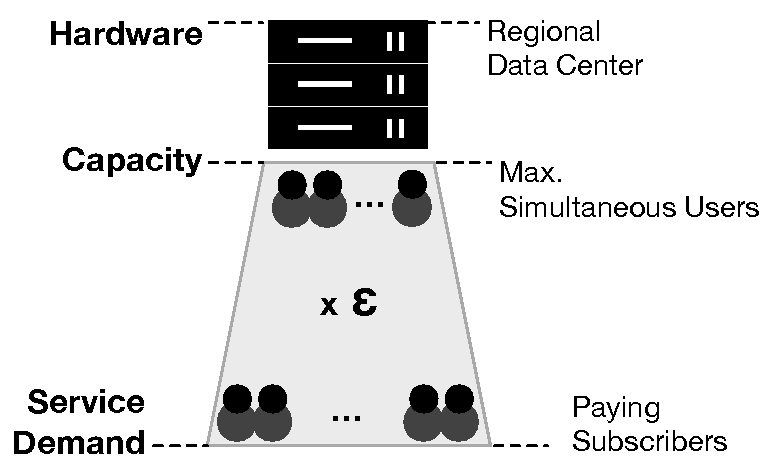
\includegraphics[width=0.65\columnwidth]{images/overbooking_datacenter.pdf}
	\caption{Overbooking of available computational capacity.}
\label{fig:overbooking_datacenter}
\end{figure}

The computational efficiency further considers the maximum overbooking rate $\epsilon \geq 1$, where $\epsilon = 1$ refers to no overbooking. $\epsilon$ is calculated as ratio of the peak utilization $d_{peak}$ (number of peak time users) from the overall capacity $Cap$, 

\begin{equation}
	\epsilon = \frac{Cap}{d_{peak}} \quad ,
\end{equation}

where $Cap$ refers to the number of subscribed users that can be handled simultaneously by this data center. The maximum number of subscribers $d$ (maximum service demand) is, thus, given by

\begin{equation}
	 d = Cap \cdot \epsilon \quad .
\end{equation}

The average monthly customer price $\bar{p}$ aggregates the monthly subscription fee and the customer's depreciation costs for the hardware investments on a four years investment duration. We further consider a minimum profit margin $m$ of $3 \%$, which is in line with the average figure for the global game industry\footnote{\url{http://www.polygon.com/2012/10/1/3439738/the-state-of-games-state-of-aaa}} and substantially below the cloud computing figures that can range up to $16.9\%$\footnote{\url{http://www.forbes.com/sites/georgeanders/2015/04/23/amazons-web-services-delight-16-9-margins-more-joy-ahead/\#73324aa64b4e}} and potentially even higher\footnote{\url{http://www.bloomberg.com/news/articles/2015-12-02/microsoft-should-disclose-cloud-revenue-margins-ballmer-says}}.

%Global Games statistics / billion revenues 2012-2016: http://newzoo.com/infographics/global-games-market-report-infographics-2013/
% Game industry = 3%: http://www.polygon.com/2012/10/1/3439738/the-state-of-games-state-of-aaa
% Game industry in the past (2009 – average console game with margin of 40%): http://www.businessinsider.com/casual-gaming-profit-margins-near-90-2009-10?IR=T
% Profit margins in cloud computing:
%	Amazon 16.9% (2015): http://www.forbes.com/sites/georgeanders/2015/04/23/amazons-web-services-delight-16-9-margins-more-joy-ahead/#73324aa64b4e
% 	Microsoft 44% (2015) -- questionable: http://www.bloomberg.com/news/articles/2015-12-02/microsoft-should-disclose-cloud-revenue-margins-ballmer-says

\begin{align} \label{eq:computational_efficiency}
	\frac{\epsilon \cdot Cap \cdot \bar{p}}{Cap} :=& \underbrace{\frac{C_{cap}}{Cap}}_{C_{u}} \cdot m =\\
	= C_{u} = \frac{C_{cap}}{Cap} :=& \epsilon \cdot \bar{p}
\end{align}

When treating the costs of the regional data center as blackbox (operational and capital costs for the data center, and required game licensing fees), the analysis can concentrate on the required capacity and licensing cost $C_{u}$ per connected user $u$.

%\begin{equation}
%	ce = \frac{C_{cap}}{Cap} \quad .
%\end{equation}

%%%%%%%%%%%%%%%%%%%%%%%%%%%%%%%%%%%%%%%%%%%%%%%%%%%%%%%%%%%%
%SOME DATA CONSIDERATIONS:
%According to http://venturebeat.com/2014/01/15/steam-has-75-million-registered-users-third-party-steam-controllers-and-other-tidbits-from-valves-dev-days/
% Customer base of Steam was 75 Million active users in 2014. 
% %Vermutlich Nutzerzahl mittlerweile hoeher. Schaetzungen waeren also konservativ ausgerichtet.
%According to http://store.steampowered.com/stats/?l=german
% Höchststand (simultaneous): 12 406 722 Nutzer maximal, Feb 13 - Feb 15
% Peak immer abends. Niedrigster Wert bei <7.5 Mio Nutzern
% => \epsilon von 75/12,406722 = 6,0451100621
% Eigentlich, da steam wächst, > 6 eine gute Annahme. Wir könnten versuchen Schranken zu definieren.
% Wenn wir annehmen, dass Skalierung gut funktioniert, benoetigen wir keinen Buffer. Sollen wir Buffer verwenden?
%%%%%%%%%%%%%%%%%%%%%%%%%%%%%%%%%%%%%%%%%%%%%%%%%%%%%%%%%%%%

\todo[inline]{NOW LET'S ADD THE DATA. Check the 12.4 Mio. E.g. user older data. Introduce customer base data and reasoning above. Illustrate that epsilon will be around 6.}

For obtaining the required minimum margin $m$, the capacity and licensing cost per user $ce$ needs to be below XXXXXXXX Euro. Considering a capacity $Cap$ for 12.4 Mio active users, this refers to a total capacity cost $C_{Cap}$ of XXXXX Euro.

The overbooking ratio $\epsilon$ could also be increased by models fostering the off-peak usage, e.g., off-peak subscriptions that only allow access to the platform outside peak hours. When considering a substantial increase of the $\epsilon$ to $1.5$---the realistic maximum when considering the high peak time centricity of the gaming use case---, we obtain a substantially lowered $C_{u}$ requirement of 

\todo[inline]{ADD DATA}

Due to the requirement of using special hardware that is focused on the gaming use case, hardware sharing with other cloud applications seems unrealistic. Thus, we can characterise that the successful will have a maximum $C_{u}$ in the following bounds:

\todo[inline]{XXX}

This maximum does not consider that the operator may not be able to fully utilize the available capacity or may not hold the optimal game licenses at all times. Thus, in practice, the required hardware costs per subscriber have to be lower than $C_{u}$ .

\todo[inline]{NOW LET'S INTERPRET IF THAT SOUNDS LIKE A HARD THING TO DO OR NOT. AND THERE WE GO.}



